\definecolor{exxetagray}{gray}{0.75}
\definecolor{itemcolor}{RGB}{179,217,255}
\definecolor{usercolor}{RGB}{255,204,179}

\shorthandoff{"}
\chapter{Empfehlungssysteme}
\label{ch:empfehlungssysteme}
% Zeitplan in Readme

\section{Einführung}
\label{ch:empfehlungssysteme:einfuehrung}
Der Begriff des Empfehlungssystems ist im englischsprachigen Raum auch unter Bezeichnungen wie "Recommender System" \cite[S. 1]{lu:2015}, "Recommender Engine" \cite[S. 1]{panigrahi:2016} und "Recommendation System" \cite[S. 1]{ebesu:2018} verbreitet. Er wurde erstmals im Jahr 1997 von \textcite[S. 1]{resnick:1997} geprägt. Dass der Begriff gerade zu diesem Zeitpunkt entstand, ist auf die zur damaligen Zeit stark wachsende Internetnutzung und die damit verbundenen einfachen Möglichkeiten zur Sammlung und Auswertung großer Mengen an Nutzerdaten zurückzuführen \cite[S. xvii]{recommenderSystems:2016}.

Besonders bekannt für den Einsatz von Empfehlungssystemen sind große IT-Konzerne wie Amazon, Facebook, Google und Netflix \cite[S. 1]{zarzour:2018}. Diese Unternehmen nutzen Recommender Engines, um ihren Kunden personalisierte Vorschläge zu den Inhalten ihrer Plattformen anzuzeigen \cite[S. 2]{jeckmans:2013}. Häufig entfällt dabei für den Anwender vollständig die Notwendigkeit einer manuellen Suche \cite[S. 1]{comibingCareer:2013}.

Der Einsatz von Empfehlungssystemen wird in der Literatur kritisch diskutiert. Beispielsweise beobachteten \textcite[S. 17f.]{alfano:2020}, dass das Empfehlungssystem der Videostreaming-Plattform YouTube dazu tendiert, neuen Anwendern zur Verlängerung ihrer Nutzungszeit verschwörungstheoretische Inhalte auszuspielen. Eine Untersuchung von Forschern des sozialen Netzwerks Facebook kam zu dem Ergebnis, dass deren Recommender Engine Nutzern verstärkt Inhalte präsentiert, welche konform mit deren Ideologien sind \cite[S. 2]{bakshy:2015}. \textcite[S. 1ff.]{pariser:2012} prägte für diese Art der Personalisierung den Begriff der Filterblase.

Empfehlungssysteme haben aber auch einen bedeutenden Anteil am wirtschaftlichen Erfolg großer Internetplattformen. So führten beispielsweise \textcite[S. 6f.]{sharma:2015} etwa 30 Prozent des Internetverkehrs beim Online-Händler Amazon unmittelbar auf den Einsatz von Empfehlungssystemen zurück. \textcite[S. 5]{gomezuribe:2016} stellten bei einer Analyse der Streaming-Plattform Netflix fest, dass ca. 80 Prozent der Nutzungszeit auf Videos entfällt, welche Nutzern ohne vorherige Suche von einer Recommender Engine angezeigt wurden.

Um solche Vorschläge generieren zu können, suchen Empfehlungssysteme relevante Inhalte basierend auf den Präferenzen der Anwender aus \cite[S. 1]{das:2017}. Zu diesem Zweck müssen benötigte Nutzerdaten zunächst erhoben und in einer maschinell auswertbaren Struktur gespeichert werden.

\section{Zugrundeliegende Datenstruktur}
\label{ch:empfehlungssysteme:arbeitsweise}
Empfehlungssysteme können die Präferenzen ihrer Nutzer sowohl über explizite als auch implizite Rückmeldungen erfassen. Explizites Feedback erhalten Plattformen beispielsweise über abgegebene Produktbewertungen oder "Gefällt mir"-Angaben in sozialen Netzwerken. Um implizite Rückmeldungen auszuwerten, werden häufig Verhaltensweisen der Nutzer aufgezeichnet. Hierbei kann es sich beispielsweise um Suchverläufe oder die Wiedergabedauer von Videos handeln \cite[S. 3]{pu:2012}.

Das gesammelte Feedback überführen Analysten in die Struktur von Matrizen \cite[S. 11f.]{recommenderSystems:2016}. Ein Beispiel für eine Matrix mit explizit erfassten Bewertungen der Fähigkeiten von Mitarbeitern ist in Tabelle \ref{tbl:empfehlungssysteme:arbeitsweise:tbl1} dargestellt.

\begin{table}[h]
	\centering
	\begin{tabular}{c|c|c|c|c|c|c}
	 & Java & Python & MySQL & MongoDB & HDFS & Spark\\ 
	\hline
	Doe, Jane & ? & 4 & 3 & 3 & ? & ?\\
	Doe, John & 3 & ? & 2 & ? & 1 & ?\\
	Muster, Erika & ? & ? & ? & ? & 5 & 3\\
	Muster, Max & 2 & 3 & 1 & ? & ? & ?
	\end{tabular}
	\caption{Beispiel für die Matrixdarstellung von Fähigkeiten}
	\label{tbl:empfehlungssysteme:arbeitsweise:tbl1}
\end{table}

In Tabelle \ref{tbl:empfehlungssysteme:arbeitsweise:tbl1} sind in der ersten Spalte die Mitarbeiter eines Unternehmens gespeichert. Diese werden als Nutzer (User) bezeichnet. In der Kopfzeile der folgenden Spalten sind verschiedene Fähigkeiten eingetragen. Diese werden Elemente (Items) genannt. In der Mitte der Tabelle befinden sich die Bewertungen (Ratings) der Fähigkeiten jedes Nutzers \cite[S. 1f.]{strub:2016}. Im Beispiel aus Tabelle \ref{tbl:empfehlungssysteme:arbeitsweise:tbl1} wurden die expliziten Beurteilungen auf einer Skala von eins bis fünf vergeben. Diese bewerteten Matrix-Einträge werden  als beobachtet (observed) oder spezifiziert (specified) bezeichnet. Unbewertete Elemente sind mit einem Fragezeichen gekennzeichnet und werden unbeobachtet (unobserved) oder fehlend (missing) genannt \cite[S. 8]{recommenderSystems:2016}.

Zahlreiche Wissenschaftler in der Literatur sind sich einig, dass für die Empfehlung geeigneter Kandidaten für eine Stelle bzw. Projektposition ein einfacher Abgleich zwischen gesuchten und vorhandenen Fähigkeiten in der Matrix eine unzureichende Lösung darstellt \cite[S. 1]{enhancingERecruitment:2012}\cite[S. 1]{faerber:2003}\cite[S. 2]{prospect:2010} und der Komplexität der Aufgabe nicht gerecht wird \cite[S. 1]{malinowski:2008}. So kritisieren beispielsweise \textcite[S. 1f.]{mitre:2014}, dass bei einem solchen Ansatz Synonyme und verwandte Fähigkeit nicht in die Suche einbezogen werden. Um diesem Problem zu begegnen, existieren in der Literatur zahlreiche unterschiedliche Ansätze, Recommender Enginges zu implementieren. Ein verbreitetes Verfahren ist das kollaborative Filtern.
% Einer davon ist die Umsetzung eines wissensbasierten Empfehlungssystems \cite[S. 2f.]{dwivedi:2017}.

\section{Kollaboratives Filtern}
\label{ch:empfehlungssysteme:cf}
Ein Ziel von Verfahren im Bereich des kollaborativen Filterns ist das Vorhersagen unbewerteter Einträge in Tabelle \ref{tbl:empfehlungssysteme:arbeitsweise:tbl1}. Unbeobachtete Werte eines Zielnutzers werden dabei über Ähnlichkeitsberechnungen aus vergebenen Beurteilungen anderer Anwender geschlussfolgert \cite[S. 1]{su:2009}.

\textcite[S. 3]{breese:1998} unterschieden zwischen speicher- (memory-) und modellbasierten (modelbased) Algorithmen. Speicherbasierte Verfahren übertragen sämtliche Nutzer und deren Bewertungen bei der Berechnung von Empfehlungen vollständig in den Hauptspeicher des Rechners. Modellbasierte Verfahren nutzen dagegen Algorithmen aus dem Bereich des Data Minings. Diese werden genutzt, um vor dem Einsatz in der Produktivumgebung statistische Vorhersage-Modelle zu entwickeln \cite[S. 3]{breese:1998}\cite[S. 11]{schafer:2007}. In der Literatur existieren unterschiedliche Ansätze, speicher- und modellbasierte Verfahren zu implementieren.

\subsection{Speicherbasierte Verfahren}
\label{ch:empfehlungssysteme:cf:speicherbasiert}
Um speicherbasierte Verfahren zu entwickeln, werden nachbarschaftsbasierte Algorithmen eingsetzt \cite[S. 29]{recommenderSystems:2016}. Soll hierbei beispielsweise die fehlende Javabewertung von Jane Doe in Tabelle \ref{tbl:empfehlungssysteme:arbeitsweise:tbl1} vorhergesagt werden, erfolgt dies über paarweise Ähnlichkeitsberechnungen \cite[S. 2f.]{bharti:2019}. Verwenden Algorithmen dabei die Ähnlichkeiten zwischen Mitarbeitern bzw. Tabellenzeilen zur Vorhersage, werden diese als nutzerorientiert (user-oriented) bezeichnet. Greifen Verfahren dagegen auf die Gleichartigkeit zwischen Fähigkeiten bzw. Tabellenspalten zurück, werden sie elementorientiert (item-oriented) genannt \cite[S. 1f.]{duong:2018}. Laut \textcite[S. 42]{recommenderSystems:2016} liefern elementorientierte Verfahren häufig präzisere, nutzerorientierte Methoden dafür diversere Ergebnisse. Somit erwartet der Autor, dass die Vorschläge der erstgenannten Ansätze für den Nutzer relevanter erscheinen. Jedoch bemängelt er das hohe Risiko bei elementbasierten Verfahren, dass dem Anwender aufgrund der hohen Ähnlichkeit der Elemente kein einziger Vorschlag gefallen könnte, wenn eine Empfehlung unzutreffend ist.

Bei der Implementierung nachbarschaftsbasierter Verfahren kommen häufig \ac{KNN}-Algorithmen zum Einsatz \cite[S. 1]{nayak:2018}. Um diese zur Vorhersage der Javabewertung von Jane Doe anzuwenden, wird bei elementorientierten Verfahren die Ähnlichkeit zwischen Java und jeder anderen Fähigkeit bestimmt, welche Jane Doe beherrscht. Anschließend wird die durchschnittliche Bewertung der k-ähnlichsten Fähigkeiten berechnet und als Java-Beurteilung für Jane Doe eingesetzt \cite[S. 2]{hao:2013} Welchen Wert Entwickler für k verwendet sollten, kann nicht pauschal beantwortet werden. Beispielsweise ist es möglich, Verfahren aus dem Bereich des maschinellen Lernens zu verwenden, um abhängig von den vorhandenen Daten einen geeigneten Wert für k ermitteln \cite[S. 2f.]{jiang:2007}.

Bei nutzerorientierten Algorithmen wird die Gleichartigkeit zwischen Jane Doe und allen anderen Mitarbeitern berechnet. Daraufhin wird die durchschnittliche Javabeurteilung der k-ähnlichsten Mitarbeiter bestimmt. Diese wird als Bewertung für die Fähigkeit Java von Jane Doe vorhergesagt \cite[S. 2f.]{hao:2013}.

Zur Ähnlichkeitsberehnung können unterschiedliche Algorithmen wie die Jaccard-Ähnlichkeit \cite[S. 2]{bharti:2019}, die euklidische Distanz \cite[S. 3]{cheng:2013} oder die Kosinus-Ähnlichkeit \cite[S. 2]{duong:2018} verwenden werden. Beispielhaft ist in der folgenden Gleichung \ref{fig:empfehlungssysteme:cf:speicherbasiert:formel1} die Formel zur Berechnung der Kosinus-Ähnlichkeit zwischen den Vektoren A und B dargestellt \cite[S. 111]{bharti:2019}:
\begin{equation}
cos(A,B) = \frac{(\vec{A} * \vec{B})}{|\vec{A}| * |\vec{B}|} = \frac{\sum_{i=1}^n A_i * B_i}{\sqrt{\sum_{i=1}^n (A_i)^2} * \sqrt{\sum_{i=1}^n (B_i)^2}}
\label{fig:empfehlungssysteme:cf:speicherbasiert:formel1}
\end{equation}
Anstelle der Vektoren A und B können in Gleichung \ref{fig:empfehlungssysteme:cf:speicherbasiert:formel1} paarweise die Spalten/Fähigkeiten bzw. Zeilen/Mitarbeiter aus Tabelle \ref{tbl:empfehlungssysteme:arbeitsweise:tbl1} eingesetzt werden.

Gleichung \ref{fig:empfehlungssysteme:cf:speicherbasiert:formel2} zeigt die nutzerbasierte Ähnlichkeitsberechnung zwischen Jane Doe und Max Muster. Dort ist zu erkennen, dass ausschließlich Tabellenspalten in die Berechnung einbezogen werden, welche von beiden Mitarbeitern bewertet wurden \cite[S. 2f.]{hao:2013}.
\begin{equation}
	cos(Jane Doe,Max Muster) = \frac{(4*3 + 3*1)}{\sqrt{4^2 + 3^2} * \sqrt{3^2 + 1^2}} \approx \frac{15}{15,811} \approx 0,95
	\label{fig:empfehlungssysteme:cf:speicherbasiert:formel2}
\end{equation}
Wie in der folgenden Gleichung \ref{fig:empfehlungssysteme:cf:speicherbasiert:formel3} dargestellt, kann analog auch die elementbasierte Ähnlichkeit für Java und MySQL aus Tabelle \ref{tbl:empfehlungssysteme:arbeitsweise:tbl1} mittels Kosinus-Distanz berechnet werden:
\begin{equation}
	cos(Java, MySQL) = \frac{(3*2 + 2*1)}{\sqrt{3^2 + 2^2} * \sqrt{2^2 + 1^2}} \approx \frac{8}{8,063} \approx 0,992
	\label{fig:empfehlungssysteme:cf:speicherbasiert:formel3}
\end{equation}
\textcite[S. 35ff.]{recommenderSystems:2016} kritisiert an solchen Berechnungen, dass möglicher Bias die Ergebnisse verzerren kann. So könnten einzelne Mitarbeiter ihre Fähigkeiten grundsätzlich schlechter oder besser einschätzen als andere Nutzer. Aus diesem Grund empfiehlt der Autor, vor den Ähnlichkeitsberechnungen zunächst eine Mittelwert-Zentrierung auszuführen. Hierbei wird in Tabelle \ref{tbl:empfehlungssysteme:arbeitsweise:tbl1} die durchschnittliche Bewertung jedes Nutzers bestimmt und von dessen vorhandenen Beurteilungen abgezogen. Dabei entstehende negative Bewertungen müssen anschließend gegebenenfalls aus der Tabelle entfernt werden. Dieses Vorgehen ist in der Literatur auch unter der Bezeichnung Pearson Korrelation bekannt \cite[S. 3]{bharti:2019}.

Es gilt zu beachten, dass die bisher vorgestellten Algorithmen im Bereich des speicherbasierten kollaborativen Filterns anfällig für das Sparsity Problem sind \cite[S. 3f.]{grvcar:2006}. Dieses bezeichnet das Phänomen, dass in der Praxis meist für einen Bruchteil aller Elemente sehr viele Bewertungen und für einen Großteil der Items dagegen nur sehr wenige Beurteilungen vorliegen \cite[S. 8]{recommenderSystems:2016}. So stellten beispielsweise \textcite[S. 3]{mitre:2014} bei der Implementierung ihres Projekt-Empfehlungssystems fest, dass über die Hälfte der ca. 17.000 vergebenen Fähigkeiten von nur je einem Mitarbeiter angegeben wurden.
Für diese Häufigkeitsverteilung prägte \textcite[S. 12]{anderson:2007} den Begriff des langen (Ratten-)Schwanzes (Long Tail). Erkennbar wird dieser, wenn Bewertungen, wie in Abbildung \ref{fig:empfehlungssysteme:cf:speicherbasiert:abb1} dargestellt, in Form eines Diagramms aggregiert werden.

\begin{figure}[h]
	\centering
	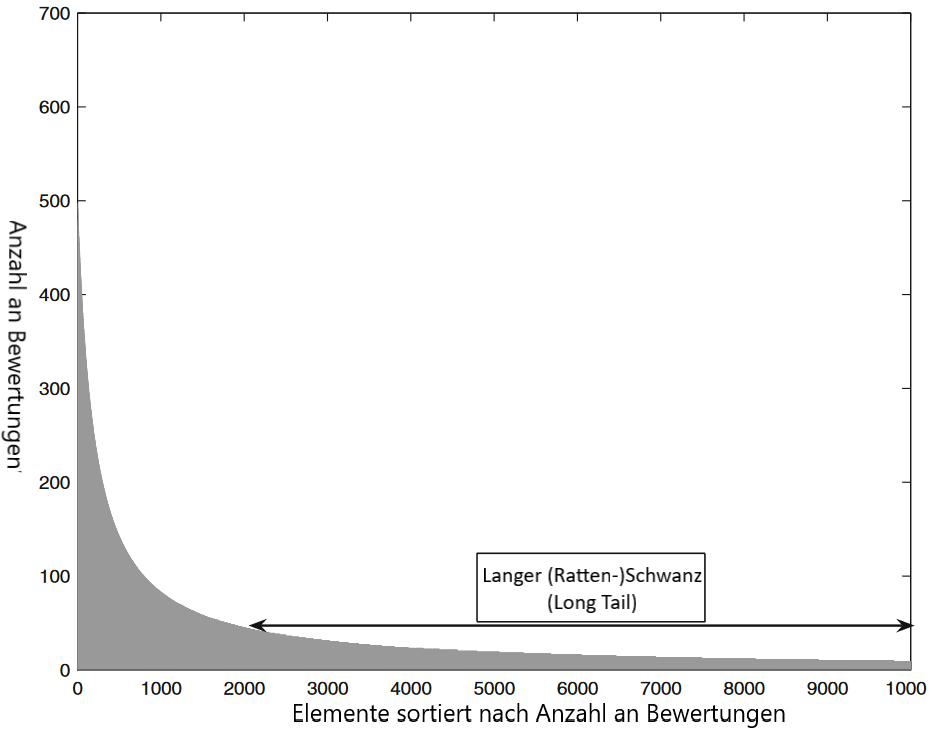
\includegraphics[width=1\textwidth]{gfx/long-tail.png}
	\caption{Darstellung des Long Tails \cite[S. 33]{recommenderSystems:2016}}
	\label{fig:empfehlungssysteme:cf:speicherbasiert:abb1}
\end{figure}

Die in Abbildung \ref{fig:empfehlungssysteme:cf:speicherbasiert:abb1} dargestellte Häufigkeitsverteilung von abgegebenen Bewertungen spiegelt \textcite[S. 1ff.]{anderson:2007} zu Folge einen allgemeinen Trend wider, welchen er im Zusammenhang mit der Digitalisierung beobachtet. Der Autor stellt fest, dass sich Menschen aufgrund der heute verfügbaren breiten Angebote wesentlich diverser orientieren, als es vor einigen Jahrzehnten der Fall war.

Das Sparsity Problem kann auch in Tabelle \ref{tbl:empfehlungssysteme:arbeitsweise:tbl1} beobachtet werden. Dort haben MongoDB und Spark jeweils nur eine Bewertung. Für diese Fähigkeiten ist es über Ähnlichkeitsberechnungen im Bereich des speicherbasierten kollaborativen Filterns somit nicht möglich, für alle Angestellten robuste Vorhersagen zu ermitteln.

Um diesem Problem zu begegnen, kann die bisher verwendete Matrixdarstellung in die Form eines bipartiten Graphen überführt werden \cite[S. 2f.]{huang:2004}. Diese Datenstruktur zeichnet sich durch die Verwendung zwei unterschiedlicher Arten von Knoten zur separaten Speicherung von Nutzern und Elementen aus. Bewertungen werden bei dieser Darstellungsform über gewichtete Kanten im Graphen dargestellt \cite[S. 1f.]{cao:2021}.

Abbildung \ref{fig:empfehlungssysteme:cf:speicherbasiert:abb2} zeigt die Fähigkeitsmatrix aus Tabelle \ref{tbl:empfehlungssysteme:arbeitsweise:tbl1} in der Datenstruktur eines bipartiten Graphen. In der Grafik sind die Knoten der Mitarbeiter rot und die Knoten der Fähigkeiten blau markiert.

\begin{figure}[h]
	\centering	
	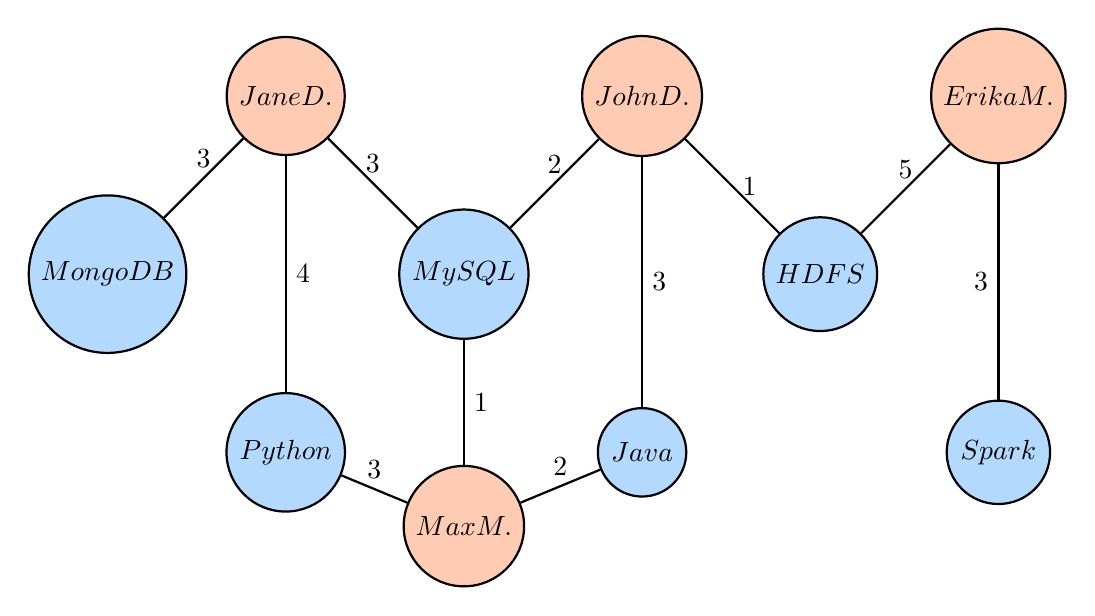
\begin{tikzpicture}[node distance={32mm}, thick, main/.style = {draw, circle}] 
		\node[main, fill=itemcolor] (MongoDB) {$MongoDB$}; 
		\node[main, fill=itemcolor] (Python) [below right of=MongoDB] {$Python$}; 
		\node[main, fill=itemcolor] (MySQL) [above right of=Python] {$MySQL$}; 
		\node[main, fill=itemcolor] (Java) [below right of=MySQL] {$Java$}; 
		\node[main, fill=itemcolor] (HDFS) [above right of=Java] {$HDFS$}; 
		\node[main, fill=itemcolor] (Spark) [below right of=HDFS] {$Spark$};
		
		\node[main, fill=usercolor] (Jane) [above right of=MongoDB] {$Jane D.$}; 
		\node[main, fill=usercolor] (John) [above left of=HDFS] {$John D.$}; 
		\node[main, fill=usercolor] (Max) [below of=MySQL] {$Max M.$};
		\node[main, fill=usercolor] (Erika) [above right of=HDFS] {$Erika M.$}; 
		
		\draw (Jane) -- node[midway, right] {4} (Python);
		\draw (Jane) -- node[midway, above] {3} (MySQL);
		\draw (Jane) -- node[midway, above] {3} (MongoDB);

		\draw (John) -- node[midway, right] {1} (HDFS);		
		\draw (John) -- node[midway, right] {3} (Java);
		\draw (John) -- node[midway, above] {2} (MySQL);
		
		%\path (Erika) edge[bend right=10] node[midway, right] {5} (HDFS); 
		\draw (Erika) -- node[midway, above] {5} (HDFS);
		\draw (Erika) -- node[midway, left] {3} (Spark);
		
		\draw (Max) -- node[midway, above] {2} (Java);
		\draw (Max) -- node[midway, above] {3} (Python);
		\draw (Max) -- node[midway, right] {1} (MySQL);
	\end{tikzpicture}

	\caption{Darstellung der Fähigkeitsmatrix aus Tabelle \ref{tbl:empfehlungssysteme:arbeitsweise:tbl1} in der Datenstruktur eines Graphen}
	\label{fig:empfehlungssysteme:cf:speicherbasiert:abb2}
\end{figure}

\textcite[S. 7ff.]{huang:2004} bemerken mit Blick auf bipartite Graphen, dass bei klassischen nachbarschaftsbasierten Algorithmen nur Empfehlungen für Knoten bestimmt werden können, welche von einem Zielknoten über drei Kanten zu erreichen sind. Somit könnten in der vorliegenden Abbildung \ref{fig:empfehlungssysteme:cf:speicherbasiert:abb2} über solche Verfahren beispielsweise keine Bewertungsvorhersagen für Jane Doe und Spark oder Erika Muster und MongoDB bestimmt werden.

Um auch in solchen Fällen Empfehlungen zu generieren, ist der Einsatz graphenbasierter Algorithmen empfehlenswert. Diese können über transitive Verbindungen auch weiter entfernte Knoten in die Berechnung mit einbeziehen \cite[S. 60f.]{recommenderSystems:2016}.

Ein in der Literatur häufig angewendeter Graphenalgorithmus ist die Katz-Zentralität \cite[S. 1ff.]{zhan:2017}\cite[S. 6]{guns:2014}\cite[S. 1f.]{huang:2004}. Diese basiert auf einem im Jahr 1953 vorgestellten mathematischen Verfahren von \textcite[S. 1ff.]{katz:1953}. Dieses entwickelte der der Wissenschaftler zur Bestimmung von Anführern in sozialen Gruppen. Heute nutzen graphenbasierte Empfehlungssysteme die Katz-Zentralität unter anderem zur Verbindungsvorhersage (Link Prediction). Diese Problemstellung ist beispielsweise im Bereich der sozialen Netzwerke verbreitet. Sie verfolgt das Ziel, aus vorhandenen Kanten im Graphen bisher unbekannte Verbindungen vorherzusagen \cite[S. 1ff.]{libenNowell:2007}.

Nah verwandt mit der Katz-Zentralität ist Googles PageRank-Algorithmus \cite[S. 1]{was:2018}. Dieser nutzt Kanten zur Darstellung von Verlinkungen im Internet. Auf dieser Grundlage bestimmte Google in seiner Anfangszeit die Wichtigkeit von Webseiten, welche in den Ergebnissen der Suchmaschine entsprechend priorisiert ausgegeben wurden \cite[S. 3ff.]{page:1999}.

Die Katz-Zentralität kann über folgende Gleichung \ref{frml:empfehlungssysteme:cf:speicherbasiert:formel4} bestimmt werden \cite[S. 4]{libenNowell:2007}:
\begin{equation}
	(I - \beta * M)^{-1} - I
	\label{frml:empfehlungssysteme:cf:speicherbasiert:formel4}
\end{equation}
In Gleichung \ref{frml:empfehlungssysteme:cf:speicherbasiert:formel4} steht $\beta$ für eine Zahl im Bereich von null bis eins \cite[S. 6]{guns:2014}, welche jedoch stets kleiner als $\frac{1}{\lambda}$ sein muss. $\lambda$ entspricht dabei dem größten Eigenwert der Matrix M \cite[S. 6]{zhan:2017}. Je größer der Wert von $\beta$ angesetzt wird, desto stärker werden weit entfernte Beziehungen in der Berechnung gewichtet \cite[S. 6]{guns:2014}.

Die Variable $M$ steht in Gleichung \ref{frml:empfehlungssysteme:cf:speicherbasiert:formel4} für die Adjazenzmatrix des betrachteten Graphen \cite[S. 4]{libenNowell:2007}. Diese gibt an, wie viele Kanten von einem Knoten (Zeile) zu jedem anderen Knoten (Spalte) führen \cite[S. 6]{guns:2014}.

Der mit Zahlen versehene Bereich von Tabelle \ref{tbl:empfehlungssysteme:arbeitsweise:tbl2} entspricht der Adjazenzmatrix für den Graphen aus Abbildung \ref{fig:empfehlungssysteme:cf:speicherbasiert:abb2}.

\begin{table}[h]
	\centering
	\begin{tabular}{c|c|c|c|c|c|c|c|c|c|c}
		& \begin{sideways}Jane D.\end{sideways} & \begin{sideways}John D.\end{sideways} & \begin{sideways}Erika M.\end{sideways} & \begin{sideways}Max M.\end{sideways} & \begin{sideways}Java\end{sideways} & \begin{sideways}Python\end{sideways} & \begin{sideways}MySQL\end{sideways} & \begin{sideways}MongoDB\end{sideways} & \begin{sideways}HDFS\end{sideways} & \begin{sideways}Spark\end{sideways} \\
		\hline
		Jane D.  & 0 & 0 & 0 & 0 & 0 & 4 & 3 & 3 & 0 & 0\\
		John D.  & 0 & 0 & 0 & 0 & 3 & 0 & 2 & 0 & 1 & 0\\
		Erika M. & 0 & 0 & 0 & 0 & 0 & 0 & 0 & 0 & 5 & 3\\
		Max M.   & 0 & 0 & 0 & 0 & 2 & 3 & 1 & 0 & 0 & 0\\
		Java     & 0 & 3 & 0 & 2 & 0 & 0 & 0 & 0 & 0 & 0\\
		Pyhton   & 4 & 0 & 0 & 3 & 0 & 0 & 0 & 0 & 0 & 0\\
		MySQL    & 3 & 2 & 0 & 1 & 0 & 0 & 0 & 0 & 0 & 0\\
		MongoDB  & 3 & 0 & 0 & 0 & 0 & 0 & 0 & 0 & 0 & 0\\
		HDFS     & 0 & 1 & 5 & 0 & 0 & 0 & 0 & 0 & 0 & 0\\
		Spark    & 0 & 0 & 3 & 0 & 0 & 0 & 0 & 0 & 0 & 0
	\end{tabular}
	\caption{Anzahl an Verbindungen im Graphen aus Abbildung \ref{fig:empfehlungssysteme:cf:speicherbasiert:abb2}}
	\label{tbl:empfehlungssysteme:arbeitsweise:tbl2}
\end{table}

%Der mit Zahlen versehene Bereich von Tabelle \ref{tbl:empfehlungssysteme:arbeitsweise:tbl2} entspricht der Adjazenzmatrix des Graphen aus Abbildung \ref{fig:empfehlungssysteme:cf:speicherbasiert:abb2}.

Für Tabelle \ref{tbl:empfehlungssysteme:arbeitsweise:tbl2} ergeben sich mit $\beta = 0.125$ durch Bestimmung der Katz-Zentralität die in Tabelle \ref{tbl:empfehlungssysteme:arbeitsweise:tbl3} dargestellten Werte. Die vollständige Berechnung kann in Appendix \ref{ch:nebenrechnungen:katzZentralitaet} nachvollzogen werden.
\newpage
\begin{table}[h]
	\centering
	\begin{tabular}{c|c|c|c|c|c|c|c|c|c|c}
		& \begin{sideways}Jane D.\end{sideways} & \begin{sideways}John D.\end{sideways} & \begin{sideways}Erika M.\end{sideways} & \begin{sideways}Max M.\end{sideways} & \begin{sideways}Java\end{sideways} & \begin{sideways}Python\end{sideways} & \begin{sideways}MySQL\end{sideways} & \begin{sideways}MongoDB\end{sideways} & \begin{sideways}HDFS\end{sideways} & \begin{sideways}Spark\end{sideways} \\ 
		\hline
		Jane D.  & 1.66 & 0.47 & 0.08 & 0.87 & 0.39 & 1.66 & 1.22 & 1.00 & 0.11 & 0.03\\
		John D.  & 0.47 & 0.42 & 0.24 & 0.37 & 0.62 & 0.37 & 0.58 & 0.18 & 0.33 & 0.09\\
		Erika M. & 0.08 & 0.24 & 1.17 & 0.06 & 0.10 & 0.06 & 0.10 & 0.03 & 1.39 & 0.81\\
		Max M.   & 0.87 & 0.37 & 0.06 & 0.60 & 0.54 & 1.04 & 0.62 & 0.33 & 0.08 & 0.02\\
		Java     & 0.39 & 0.62 & 0.10 & 0.54 & 0.37 & 0.40 & 0.37 & 0.15 & 0.14 & 0.04\\
		Pyhton   & 1.66 & 0.37 & 0.06 & 1.04 & 0.40 & 1.22 & 0.84 & 0.62 & 0.09 & 0.02\\
		MySQL    & 1.22 & 0.58 & 0.10 & 0.62 & 0.37 & 0.84 & 0.68 & 0.46 & 0.13 & 0.04\\
		MongoDB  & 1.00 & 0.18 & 0.03 & 0.33 & 0.15 & 0.62 & 0.46 & 0.37 & 0.04 & 0.01\\
		HDFS     & 0.11 & 0.33 & 1.39 & 0.08 & 0.14 & 0.09 & 0.13 & 0.04 & 0.91 & 0.52\\
		Spark    & 0.03 & 0.09 & 0.81 & 0.02 & 0.04 & 0.02 & 0.04 & 0.01 & 0.52 & 0.31
	\end{tabular}
	\caption{Berechnete Katz-Zentralität mit $\beta = 0.125$ für Tabelle \ref{tbl:empfehlungssysteme:arbeitsweise:tbl2}}
	\label{tbl:empfehlungssysteme:arbeitsweise:tbl3}
\end{table}

In Tabelle \ref{tbl:empfehlungssysteme:arbeitsweise:tbl3} ist zu erkennen, dass durch Bestimmung der Katz-Zentralität für sämtliche Knoten die Stärke der Verbindung zu allen anderen Knoten vorhergesagt werden konnte. Das Sparsity Problem wurde somit behoben. Die vorliegenden Ergebnisse eigenen sich folglich sehr gut, um auf deren Basis Ähnlichkeiten zwischen Nutzern oder Fähigkeiten zu bestimmen.

Allerdings ist auch festzustellen, dass die Skalierung der Bewertungen verändert wurde. Projekt-Anforderungen, welche auf der in Tabelle \ref{tbl:empfehlungssysteme:arbeitsweise:tbl2} verwendeten Bewertungsskala spezifiziert wurden, könnte ein Algorithmus somit nicht ohne weiteres mit den Ergebnissen aus Tabelle \ref{tbl:empfehlungssysteme:arbeitsweise:tbl3} abgleichen.

Eine Lösungsmöglichkeit zeigen Algorithmen von Gruppen-Recommender Engines auf. Solche Systeme verfolgen das Ziel, gemeinsame Vorschläge für mehrere Anwender zu generieren \cite[S. 1]{dara:2020}. Ein in diesem Zusammenhang angewendetes Verfahren ist das Erstellen eines Pseudonutzers, welcher die Präferenzen aller Gruppenmitglieder vereint. Der Pseudonutzer wird bei Empfehlungsberechnung als gewöhnlicher Anwender betrachtet und beispielsweise in Tabelle \ref{tbl:empfehlungssysteme:arbeitsweise:tbl1} in eine neue Zeile eingefügt. Dieses Vorgehen ermöglicht es, die bisher vorgestellten Verfahren im Bereich des kollaborativen Filterns ohne zusätzlich Komplexität auch zur Bestimmung von Vorschlägen für Gruppen anzuwenden \cite[S. 8f.]{oconnor:2001}.

Ein vergleichbarer Ansatz könnte auch bei der Bestimmung der Katz-Zentralität genutzt werden. Hierfür müsste ein Algorithmus zunächst Tabelle \ref{tbl:empfehlungssysteme:arbeitsweise:tbl2} um eine Zeile erweitern, in welcher das zu besetzende Projekt mitsamt den dafür benötigten Fähigkeiten als Pseudo-Mitarbeiter einfügt wird. Nach der anschließenden Bestimmung der Katz-Zentralität würden auch die Fähigkeiten des Pseudomitarbeiters der neuen Skalierung entsprechen. Somit könnten diese neuen Fähigkeitsbewertungen als Ausgangspunkt für die Bestimmung passender Mitarbeiter für das Projekt verwendet werden. Ein vergleichbares Verfahren wendeten auch \textcite[S. 2]{mitre:2014} bei der Implementierung ihres Empfehlungssystems zur Projektbesetzung an. Die Wissenschaftler nutzen jedoch klassische Verfahren zur Ähnlichkeitsberechnung und keine Graphenalgorithmen.

Unabhängig von der konkreten Art der Implementierung ist ein großer Nachteil an speicherbasierten Verfahren, dass bei jeder Empfehlungsberechnung sämtliche Nutzer, Elemente und Bewertungen in den Hauptspeicher geladen werden müssen \cite[S. 8]{yang:2016}. Zusätzlich ist festzustellen, dass häufig sehr hohe Laufzeiten zu erwarten sind \cite[S. 2]{zhang:2010}. So bemerken beispielsweise \textcite[S. 3]{landherr:2010}, dass alleine die Matrix-Invertierung zur Bestimmung der Katz-Zentralität mit Gleichung \ref{frml:empfehlungssysteme:cf:speicherbasiert:formel4} eine Komplexität von $O(n^3)$ besitzt. Aus diesen Gründen ist die Verwendung speicherbasierter Ansätze bei großen Datensätzen als ungeeignet zu bewertet. Abhilfe bei steigender Datenmenge können modellbasierte Verfahren bieten.

\subsection{Modellbasierte Verfahren}
\label{ch:empfehlungssysteme:cf:modellbasiert}
Modellbasierte Verfahren verwenden Ansätze aus dem Bereich des Data Minings zur Generierung von Vorschlägen. Hierbei berechnen Wissenschaftler statistische Modelle, bevor sie ihr Empfehlungssystem den Nutzern zur Verfügung stellen \cite[S. 2]{cui:2020}. Dieses Vorgehen hat den Vorteil, dass in der Produktivumgebung keine Berechnungen mehr auf allen Daten ausgeführt werden müssen. Somit ist die Vorschlagsbestimmung insbesondere bei großen Datenmengen effizienter als bei speicherbasierten Verfahren \cite[S. 8]{yang:2016}.

Wie in Tabelle \ref{tbl:empfehlungssysteme:cf:modellbasiert:tbl1} dargestellt, ist es bei modellbasierten Verfahren üblich, den vorhandenen Datensatz in Trainings- (rot) und Testdaten (blau) zu untergliedern \cite[S. 71f.]{recommenderSystems:2016}. Die Einteilung erfolgte hierbei zufällig.%Bei Modellentwicklungen zur Vervollständigung von Matrizen nutzen Wissenschaftler häufig die beobachteten Felder als Trainings- und die unbeobachteten Einträge als Testdaten \cite[S. 71f.]{recommenderSystems:2016}. Die Aufteilung kann beispielsweise im Verhältnis von 80 Prozent Trainings- und 20 Prozent Testdaten erfolgen \cite[S. 12]{najafabadi:2017}. 

\begin{table}[h]
	\centering
	\begin{tabular}{c|c|c|c|c|c|c}
		& Java & Python & MySQL & MongoDB & HDFS & Spark\\ 
		\hline
		Doe, Jane 		& \cellcolor{itemcolor}2 & \cellcolor{usercolor}4 & \cellcolor{itemcolor}3 & \cellcolor{usercolor}3 & \cellcolor{itemcolor}2 & \cellcolor{usercolor}1\\
		Doe, John 		& \cellcolor{usercolor}3 & \cellcolor{itemcolor}4 & \cellcolor{usercolor}2 & \cellcolor{itemcolor}1 & \cellcolor{usercolor}1 & \cellcolor{itemcolor}3\\
		Muster, Erika 	& \cellcolor{itemcolor}5 & \cellcolor{usercolor}2 & \cellcolor{itemcolor}3 & \cellcolor{usercolor}2 & \cellcolor{usercolor}5 & \cellcolor{usercolor}3\\
		Muster, Max 	& \cellcolor{usercolor}2 & \cellcolor{usercolor}3 & \cellcolor{usercolor}1 & \cellcolor{itemcolor}4 & \cellcolor{usercolor}1 & \cellcolor{itemcolor}2
	\end{tabular}
	\caption{Beispiel für eine Matrixdarstellung von Fähigkeiten mit Unterteilung in Trainings- und Testdaten}
	\label{tbl:empfehlungssysteme:cf:modellbasiert:tbl1}
\end{table}

Die Trainingsdaten werden genutzt, um statistische Modelle zur Vorhersage von Bewertungen zu entwickeln \cite[S. 71f.]{recommenderSystems:2016}.  Diese werden anschließend durch die Testdaten evaluiert und hinsichtlich der Genauigkeit der Vorhersagen bewertet. Hierbei ist es beispielsweise möglich, bekannte Einträge in der Matrix temporär zu entfernen, diese anschließend durch das trainierte Modell vorherzusagen und daraufhin tatsächliche und vorhergesagte Werte zu vergleichen \cite[S. 3ff.]{kang:2016}.
% die Implementierung neuronaler Netze \cite[S. 5ff.]{personJobFit:2018}, die Anwendung des naiven Bayes-Klassifikators \cite[S. 2]{valdividezodiaz:2019}, die Durchführung von Matrix-Faktorisierungsverfahren \cite[S. 2ff.]{ortega:2016} oder die Berechnung von Entscheidungsbäumen \cite[S. 1ff.]{yu:2012} verbreitet.

Wie an den Spalten in Tabelle \ref{tbl:empfehlungssysteme:cf:modellbasiert:tbl1} zu erkennen ist, existieren in der Praxis häufig sehr viele Merkmale bzw. Dimensionen, welche zur Entwicklung von Modellen relevant sein können. Zusätzlich sind Matrizen, wie in Kapitel \ref{ch:empfehlungssysteme:cf:speicherbasiert} beschrieben, in der Praxis aufgrund des Sparsity Problems meist sehr schwach besetzt. \textcite[S. 1]{boratto:2014} stellen fest, dass in solchen Situationen, in welchen viele Dimensionen und gleichzeitig wenigen Daten vorliegen, keine statistisch aussagekräftigen Modelle erstellt werden können. \textcite[S. 94]{bellman:1961} prägte für diesen Sachverhalt den Ausdruck "Fluch der Dimensionalität"\footnote{"Curse of dimensionality" - \textcite[S. 94]{bellman:1961}}. Um in solchen Situationen dennoch Empfehlungen generieren zu können, stellen verschiedene Autoren in der Literatur Verfahren zur Dimensionsreduzierung vor. Verbreitet ist dabei beispielsweise die Hauptkomponentenanalyse, welche im englischsprachigen Raum als \ac{PCA} bezeichnet wird \cite[S. 1ff.]{vaswani:2018}.

\textcite[S. 1f.]{pennock:2000} kritisieren an modellbasierten Verfahren, dass diese stets den Zustand der Daten zum Zeitpunkt des Trainings des Modells abbilden. Werden beispielsweise Fähigkeiten in der Datenbank hinzugefügt bzw. entfernt oder Bewertungen signifikant verändert, muss gegebenenfalls das statistische Modell neu trainiert werden, um diese Anpassungen zu erfassen. Speicherbasierte Verfahren können den Autoren zu Folge solche Änderungen dagegen unmittelbar berücksichtigen.

Ein Problem, welches weder speicher- noch modellbasierte Verfahren im Bereich des kollaborativen Filterns zuverlässig lösen können, ist der sogenannte Kaltstart (Cold Start). Dieser tritt auf, wenn neue Nutzer oder Fähigkeiten in die Datenbank hinzugefügt werden, welchen noch keine Bewertung zugeordnet ist \cite[S. 5]{huang:2004}. In solchen Fällen ist die gesamte Zeile bzw. Spalte in Tabelle \ref{tbl:empfehlungssysteme:arbeitsweise:tbl1} mit fehlenden Einträgen gekennzeichnet. Im entsprechenden Graphen in Abbildung \ref{fig:empfehlungssysteme:cf:speicherbasiert:abb2} existiert somit keine Kante von der betrachteten Entität zu anderen Knoten. Daher ist es weder über speicherbasierte Ähnlichkeitsberechnungen, noch mittels graphenbasierter Algorithmen oder statistischen Modellen möglich, zuverlässige Vorhersagen zu bestimmen. Eine Lösung für den Kaltstart können jedoch Verfahren im Bereich des inhaltsbasierten Filterns bieten.

\section{Inhaltsbasiertes Filtern}
\label{ch:empfehlungssysteme:inhaltsbasiertesFiltern}
Verfahren des inhaltsbasierten Filterns nutzen im Unterschied zum kollaborativen Filtern keine Daten anderer Anwender zur Bestimmung von Vorhersagen. Algorithmen in diesem Bereich fokussieren Beschreibungen von Nutzern und Elementen \cite[S. 139f.]{recommenderSystems:2016}.

Soll analog zum Beispiel aus Kapitel \ref{ch:empfehlungssysteme:cf:speicherbasiert} die Javabewertung von Jane Doe vorhergesagt werden, würden beim inhaltsbasierten Filtern somit keine Ähnlichkeitsberechnungen zwischen Java und jeder anderen Fähigkeit bzw. Jane Doe und allen anderen Mitarbeitern durchgeführt werden. Stattdessen könnten beispielsweise Satzbausteine im Lebenslauf von Jane Doe mit Wörtern in entsprechender Fachliteratur zu Javatechnologien verglichen werden.

Solche Anwendungen im Bereich des inhaltsbasierten Filterns implementierten beispielsweise \textcite[S. 4ff.]{guo:2016} und \textcite[S. 3ff.]{prospect:2010}. Diese entwickelten Empfehlungssysteme zur Stellensuche bzw. -besetzung. In beiden Fällen nutzten die Wissenschaftler Methoden aus der Computerlinguistik, um aus unstrukturierten Stellenausschreibungen und Lebensläufen semantische Merkmale zu extrahieren. Die dabei gewonnenen Daten speicherten sie einer strukturierten Form, welche den Forschern die Anwendung von Ähnlichkeitsberechnungen ermöglichte. Über diese bestimmten \textcite[S. 4ff.]{guo:2016} die Übereinstimmungen im Lebenslauf eines Anwenders mit vorhandenen Stellenbeschreibungen in deren Datenbank. Die dabei ermittelten relevantesten Gesuche wurden an den Nutzer zurückgegeben. Ähnlich arbeitete auch das Empfehlungssystem von \textcite[S. 3ff.]{prospect:2010}. Diese bestimmten die Ähnlichkeit zwischen den Lebensläufen von Bewerbern und einer zu besetzenden Stelle, um Personalsachbearbeiter bei der Kandidatenauswahl zu unterstützen.

Diesen Ansatz verfolgten auch \textcite[S. 1ff.]{almalis:2014}, um ein inhaltsbasiertes Empfehlungssystem zu entwickeln, welches geeignetes Personal für offene Stellen bestimmte. Hierbei überführten Sie unstrukturierte Stellenanforderungen und Lebensläufe der Kandidaten in die Form einheitlicher Vektoren. Über Ähnlichkeitsberechnungen bestimmten die Wissenschaftler diejenigen Personen, welche die höchste Übereinstimmung mit den gesuchten Anforderungen aufweisen konnten.

Auch ist es möglich, graphenbasierte Verfahren im Bereich des inhaltsbasierten Filterns  einzusetzen. Diese bieten die Möglichkeit, vorhandene Daten über Ontologien miteinander zu verbinden. So entwickelten beispielsweise \textcite[S. 1ff.]{kumaran:2013} ein IT-System, welches Bewerbungen und Stellenausschreibungen über Verfahren der Computerlinguistik in einheitliche Ontologien überträgt. Auch hier ermittelten die Wissenschaftler über Ähnlichkeitsberechnungen die geeignetsten Bewerber für offene Stellen.

Es wäre ebenso denkbar, die von \textcite[S. 1ff.]{kumaran:2013} entwickelten Ontologien um weiteres Domänenwissen anzureichern und dieses in den Vorschlagsprozess einzubeziehen. Ein solches Vorgehen verfolgen wissensbasierte Empfehlungssysteme \cite[S. 168f.]{recommenderSystems:2016}.% Da auch diese Anwendungen Vorschläge auf Basis der Eigenschaften von Nutzern und Elementen generieren, wird in der Literatur diskutiert, ob es sich bei wissens- und inhaltsbasierten Empfehlungssystemen um separate Gattungen von Recommender Engines handelt.

\section{Wissensbasierte Empfehlungssysteme}
\label{ch:empfehlungssysteme:wissensbasierteAnsaetze}
% Anmerkung Andreas (21. Juni): Esco ist sehr allgemein
Beim Erstellen von wissensbasierten Empfehlungssystemen können Unternehmen auf bereits vorhandene Ontologien zurückgreifen. Beispielsweise stellt die Europäische Kommission mit \acs{ESCO} (\acl{ESCO}) explizit zum Zweck der Stellenbesetzung eine mehrsprachige Ontologie mit vordefinierten Kompetenzen, Fähigkeiten und Qualifikationen bereit \cite[S. 1ff.]{leVrang:2014}. Ein vergleichbares Angebot existiert mit \acs{ONet} (\acl{ONet}) auch von der Regierung der Vereinigten Staaten von Amerika \cite[S. 2]{aCombinedRepresentation:2018}.

In solchen Wissensdatenbanken können Unternehmen zu Stellen passende Mitarbeiter über semantische Suchen abfragen. Hierbei kann das System über hinterlegte Regeln sowohl Synonyme als auch Beziehungen berücksichtigen \cite[S. 2f.]{singto:2013}. Jedoch werden dabei Mitarbeiter in den Ergebnissen nur ausgegeben, wenn sie die Suchanfrage exakt erfüllen. Aus diesem Grund stellen \textcite[S. 3]{bianchini:2008} bei semantischen Suchen eine hohe Genauigkeit der Resultate fest, bemängelten jedoch die Flexibilität der Verfahren.

Auch ist es möglich, innerhalb der Ontologien über Graphenalgorithmen die Übereinstimmungen zwischen Fähigkeiten zu berechnen \cite[S. 1f.]{balachander:2018}. Bei solchen, auf Ähnlichkeitsberechnungen basierenden Verfahren, beobachteten \textcite[S. 4]{bianchini:2008} eine hohe Flexibilität, kritisierten jedoch die mangelnde Genauigkeit der Verfahren.

Um die Nachteile beider Ansätze auszugleichen, implementierten \textcite[S. 4ff.]{semanticMatchmaking:2009} ein eigenes Empfehlungssystem. Dieses sollte gleichzeitig eine hohe Genauigkeit und Flexibilität gewährleisten. Für dieses Vorhaben entwickelten die Wissenschaftler eine Ontologie, welche die Fähigkeiten der Mitarbeiter sehr feingranular erfasst. Einzelne Kompetenzen mussten dabei über mehrere Einträge spezifiziert werden. Zu Stellen passende Personen wurden anschließend über einen Algorithmus ermittelt, welcher semantische Schlussfolgerungen mit Ähnlichkeitsberechnungen kombinierte. Mit diesem Ansatz erreichten \textcite[S. 11f.]{semanticMatchmaking:2009} ihr Ziel, ein genaues und zugleich flexibles wissensbasiertes Empfehlungssystem zu implementieren. Jedoch muss kritisch angemerkt werden, dass die Pflege der Fähigkeiten in der Ontologie als sehr aufwändig erscheint. Somit muss in Frage gestellt werden, ob Mitarbeiter ein solches System zuverlässig im Unternehmensalltag pflegen würden. Auch \textcite[S. 2]{aCombinedRepresentation:2018} beobachten in anderen Job-Ontologien wie \acs{ONet}, dass Informationen über Fähigkeiten häufig nicht aktuell gehalten werden.

Die von \textcite[S. 1]{semanticMatchmaking:2009} implementierte Recommener Engine kombinierte semantische Schlussfolgerungen und Ähnlichkeitsberechnungen in einem System. Aus diesem Grund kann deren Anwendung auch als hybrides Empfehlungssystem bezeichnet werden.

\section{Hybride Empfehlungssysteme}
\label{ch:empfehlungssysteme:hybrideEmpfehlungssysteme}
Hybride Systeme verwenden innerhalb einer Anwendung mehrere unterschiedliche Empfehlungsansätze. Dadurch können sie die Nachteile einzelner Verfahren ausgleichen bzw. die Vorteile mehrerer Ansätze miteinander verbinden, um die Qualität der Ergebnisse zu verbessern \cite[S. 199f.]{recommenderSystems:2016}\cite[S. 8]{malinowski:2008}.

Beispielsweise entwickelten \textcite[S. 1ff.]{shalaby:2017} ein hybrides Empfehlungssystem für eine Website zur Stellensuche. Dabei bezogen sie mehrere Datenquellen in den Vorschlagsprozess ein und kombinierten dabei unter anderem graphen- und modellbasierte Methoden. Ihr hybrides System verglichen die Wissenschaftler in einem A/B-Test mit dem auf der Website bisher eingesetzten modellbasierten Verfahren aus dem Bereich des kollaborativen Filterns. Hierbei konnten sie nachweisen, dass die Nutzer höheres Interesse an den Stellen des hybriden Empfehlungssystems aufzeigten. Jedoch muss die Evaluation kritisch betrachtet werden. So empfahlen \textcite[S. 10f.]{stegemann:2020} bei A/B-Tests bei jeder zu testenden Variante jeweils nur ein Merkmal zu verändern. Ansonsten kann den Autoren zu Folge in der Evaluation nicht mit Sicherheit bestimmt werden, welche Anpassung zur Veränderung des Nutzerverhaltens führte. \textcite[S. 1ff.]{shalaby:2017} änderten in ihrem System jedoch mehrere Merkmale in der neuen Variante. So nutzten sie unter anderem anstelle des kollaborativen Filterns hybride Verfahren und verwendeten zusätzlich mehr Datenquellen als die vorherige Variante. Somit kann nicht mit Sicherheit festgestellt werden, dass die verbesserten Ergebnisse auf den Einsatz des hybriden Systems zurückzuführen ist. Auch wäre es denkbar, dass die Einbeziehung zusätzlicher Datenquellen zum veränderten Nutzerverhalten führte.

\textcite[S. 8]{combiningCbAndCFCostSensitiveApproach:2017} konnten durch die Implementierung hybrider Verfahren nachweisen, dass sie die Empfehlungen bei Stellensuchen verbessern konnten.

\textcite[S. 16]{hybridImmunizing:2017} zeigten, dass deren hybrides Job-Empfehlungssystem trotz der Kombination mehrerer Verfahren eine nach wie vor sehr hohe Performance aufweisen konnte.

\textcite[S. 1]{malinowski:2008} kritisierten jedoch, dass auch ein hybrides Empfehlungssystem nicht ausreicht, um geeignete Mitarbeiter für Stellen zu empfehlen. Deren Einschätzung zu Folge ist die Entwicklung bilateraler Empfehlungssysteme notwendig.



\newpage
%Hybride Recommender Engines kombinieren die Vorzüge mehrerer der bisher vorgestellten Empfehlungsverfahren innerhalb eines Systems \cite[S. 8]{malinowski:2008}. Hinsichtlich solcher Ansätze konnten beispielsweise \textcite[S. 8]{combiningCbAndCFCostSensitiveApproach:2017} nachweisen, dass sie durch die Implementierung eines hybriden Verfahrens die Empfehlungen bei Stellensuchen verbessern konnten. \textcite[S. 16]{hybridImmunizing:2017} zeigten, dass deren hybrides Job-Empfehlungssystem trotz der Kombination mehrerer Verfahren eine nach wie vor sehr hohe Performance aufweisen konnte.

%HR-Manager sollten beachten, dass ihr eingesetztes Empfehlungssystem auch einen guten Umgang mit dem Sparse Data-Problem bietet. Dieses bezeichnet das Phänomen, dass in der Praxis für einen Großteil der Fähigkeiten nur sehr wenige Bewertungen vorliegen \cite[S. 8]{recommenderSystems:2016}. So stellten \textcite[S. 3]{mitre:2014} bei der Implementierung ihres Projekt-Empfehlungssystems fest, dass über die Hälfte der ca. 17.000 vergebenen Fähigkeiten von nur je einem Mitarbeiter angegeben wurden. Um auch bei einer solch geringen Datendichte Empfehlungen generieren zu können, schlagen einige Wissenschaftler auch hier die Implementierung hybrider Verfahren vor \cite[S. 3]{weightedSimilarity:2015}.
- \cite[S. 33]{recommenderSystems:2016}: Beispiele zum kollaborativen Filtern: Kann über Nachbarschaften zwischen Nutzern (User-based Models) (Wenn Alice und Bob in der Vergangenheit ähnliche Filme bewertet haben, kann Alice Bewertung für Terminator genutzt werden, um Bobs nicht vergebene Bewertung für Terminator vorherzusagen) oder Nachbarschaft zwischen Items (Item-Based Models) --> Ähnliche Items werden vom Nutzer ähnlich bewertet --> Um Bobs Bewertung für Terminator vorherzusagen, können Bobs Bewertungen für Alien and Predator verwendet werden / Neighborhood Methoden können als Generalisierung von Nearest Neighbor Klassifikatoren aus der ML-Literatur betrachtet werden --> Unterschied: Beim Kollaborativen Filtern können Ähnlichkeiten sowohl in Spalten als auch Zeilen gefunden werden --> Bei ML nur in Rows

- \cite[S. 34f.]{recommenderSystems:2016}: User-Based Neighborhood Models: Berechne Ähnlichkeit zwischen allen Nutzern i und einem Zielnutzer u --> Dazu muss eine Ähnlichkeitsfunktion verwendet werden --> Nimm dazu für jedes Nutzer-Paar alle Items, die beide bewertet haben und berechne darüber die Ähnlichkeit --> z.B. mit Pearson Korrelations-Koeffizient --> Danach kann man ein Set mit k Nutzern auswählen, welche die höchste Ähnlichkeit aufweisen --> Durchschnitt derer Bewertungen kann zur Vorhersage genutzt werden / Achtung: Nutzer könnten unterschiedlich gut bewerten (grundsätzlich besser oder grundsätzlich schnlechter), deshalb: Bewertungen mean-centern, bevor die durchschnittliche Bewertung der Peer-Group bestimmt wird --> Mean-Centern: Durchschnittliche Bewertung eines Nutzers von der Rohbewertung des Items abziehen --> S. 39: Negative Bewertungen sollten gefiltert werden

- \cite[S. 40f.]{recommenderSystems:2016}: Item-Based Neighborhood Models: Ähnlichkeiten werden zwischen Items (Spalten) berechnet --> Erstmal mean centern --> Dann werden alle Nutzer geladen, die das Ziel-Item bewertet haben --> Ähnlichkeit berechnen z.B. Mit AdjustedCosinus (bietet hier bessere Ergebnisse als Pearson) --> Nimm top k-Items --> Gewichteten Durchschnitt berechnen (unter Einbeziehung der Bewertungen des Nutzers für Hebelwirkung)

- \cite[S. 44]{recommenderSystems:2016}: Vorteile Neighborhood: Einfacher und intuitiver Ansatz; Nachteil: Berechnung kann bei großen Datenmengen unpraktisch werden --> Kann langsam werden (vgl. Offline- Online Phase)

- \cite[S. 44]{recommenderSystems:2016}: Kombination von Item- und User-Based: Wichtig: Beide müssen denselben Algorithmus nutzen --> Zuvor mean-centern --> Für Zieleintrag ähnlichste Zeilen und Spalten bestimmen --> Für Zieleintrag die gewichtete Kombination aus den top-k ähnlichsten bestimmen

- \cite[S. 46]{recommenderSystems:2016}: Alternativ: Offline-Clustern

- \cite{recommenderSystems:2016}: Allgemeine Anmerkung: Laufzeiten O(..) wurden im Text genannt / Grundsätzlich: Hauptprobleme bei Memory-Based: Sparsity und hohe Berechnungszeit

- \cite[S. 60]{recommenderSystems:2016}: Sparsity ist ein großes Problem bei Nachbarschafts-Berechnungen  --> Graphen können helfen --> Können für Nutzer, Items oder beide Konzipiert werden --> Bestimmt auch Nachbarschaft --> Ist aber effektiver bei sparse Settings

- \cite[S. xvii]{recommenderSystems:2016}: Thema der RS erhielt eine steigende Wichtigkeit in den 90ern, als das Web ein wichtiges Medium für Wirtschaft und Online-Handel wurde --> Es wurde früh erkannt, dass das Web unerreichte Möglichkeiten zur Personalisierung bereit hielt, welche in anderen Kanälen nicht zur Verfügung standen --> Web bot einfache Datensammlung und Nutzeroberfläche, um empfohlene Items in einer unaufdringlichen Weise anzuzeigen

- \cite[S. xvii]{recommenderSystems:2016}: Bekannteste Methoden: kollaboratives filtern, inhaltsbasiertes filtern und wissensbasierte Systeme

- \cite[S. 1]{recommenderSystems:2016}: Wichtigkeit des Webs war eine treibende Kraft für die Entwicklung der RS-Technologie --> Wichtiger Katalysator: Einfachheit, mit der Nutzer Feedback über Likes und Dislikes oder Bewertungen vergeben können / Es gibt auch implizites Feedback, z.B. indem der Nutzer sich ein Element ansieht oder einkauft --> Vergangene Interaktion mit dem Item --> Diese sind oft ein guter Indikator für zukünftige Wahl

- \cite[S. 1]{recommenderSystems:2016}: Grundidee des RS: Verschiedenen Datenquellen nutzbar machen und daraus Kundeninteressen schlussfolgern

- \cite[S. 1f.]{recommenderSystems:2016}: Ausnahme: Wissensbasierte RS --> Hier werden Empfehlungen eher auf Basis von Nutzer-spezifizierten Anforderungen als auf Vergangenheitsdaten generiert

- \cite[S. 2]{recommenderSystems:2016}: Kollaboratives Filtern bedeutet die Bewertung vieler Nutzer in einem kollaborativen Weg einzubeziehen, um fehlende Bewertungen schlusszufolgern

- \cite[S. 2]{recommenderSystems:2016}: Inhaltsbasiertes Filtern: Content spielt die primäre Rolle im Empfehlungsprozess --> Bewertungen der Nutzer und Attribut-Beschreibungen werden genutzt, um Empfehlungen abzugeben

- \cite[S. 2]{recommenderSystems:2016}: Knowledge-Based: Nutzer spezifizieren Interaktiv ihre Interessen --> Nutzerspezifikation wird mit Domänenwissen kombiniert, um Empfehlungen zu generieren

- \cite[S. 3]{recommenderSystems:2016}: Zwei primäre Empfehlungsprobleme: 1. Vorhersageproblem --> Hier gibt es spezifizierte bzw. observed items und fehlende bzw. unobserved Werte --> Auch genannt: Matrix completion problem --> Ziel: fehlende Werte durch lernenden Algorithmus vorherzusagen / 2. Ranking-Version des Problems: Bestimmung der top k-Items --> Auch genannt: top-k recommendation problem --> Hier sind absolute Werte nicht wichtig; 4. Erhöhung der Empfehlungs-Diversität (Wenn alle top-k Items sehr ähnlich sind, erhöht das die Gefahr, dass sich der Nutzer für keines der Items interessiert --> Sind die Empfehlungen diverser, ist die Wahrscheinlichkeit höher, dass der Nutzer zumindest ein Item mag)

- \cite[S. 4]{recommenderSystems:2016}: Ziele: 1. Relevanz (Relevant für Nutzer); 2. Neuheit (Nutzer hat das in der Vergangenheit noch nicht gesehen --> Quelle); 3. Serendipität (Nutzer bekommt etwas vorgeschlagen, das ihn positiv überrascht) / Beispiel: Indisches Restaurant eröffnet in der Nähe von jemandem der oft indisch isst --> Das Restaurant zu empfehlen wäre Neu, aber nicht Serendipität --> Serendipität wäre, wenn der Nutzer ein ethiopisches Restaurant empfohlen bekommt / Serendipität kann langfristig zu einem neuen Interesse des Nutzers und somit zu strategischen Vorteilen für den Verkäufer führen; Führt aber auch oft zur Empfehlung irrelevanter Items

- \cite[S. 5]{recommenderSystems:2016}: GroupLens war ein Pionier-RS --> Forschungs-Prototyp für die Empfehlung von Nachrichtenartikeln

- \cite[S. 5]{recommenderSystems:2016}: Amazon (Quelle) war auch ein Pionier, insbesondere für den Handel --> Haben sehr früh die Nützlichkeit dieser Technologie erkannt; Bewertungen werden durch ein 5-Sterne-System gespeichert; Auch werden Surf-Daten geloggt / Unterscheidung explizite und implizite Bewertung 

- \cite[S. 5f.]{recommenderSystems:2016}: Streaming-Anbieter; Bietet explizit Beispiele für Empfehlungen basierend auf angesehenen Items --> Hilft dem Nutzer zu entscheiden, ob dieser den Film sehen möchte --> Hilft dem Nutzer zu verstehen, weshalb er einen bestimmten Film sehen möchte / Netlifx-Preis / Cinematch

- \cite[S. 6]{recommenderSystems:2016}: Google News (Quelle): Empfiehlt Nachrichten basiernd auf der Click-Historie / Klick auf Artikel wird als positives Feedback gewertet 

- \cite[S. 7]{recommenderSystems:2016}: Facebook: Empfiehlt potentielle Freunde --> Erhöht Vernetzung und Wachstum des sozialen Netzwerks

- \cite[S. 8]{recommenderSystems:2016}: Zwei Arten von Daten: 1. Nutzer-Item Interaktionen (genutzt für Kollaboratives Filtern) und Attribut-Informationen (genutzt für Content-Based --> nutzen auch Bewertungen, aber von einem einzigen Nutzer und nicht von allen)

- \cite[S. 8]{recommenderSystems:2016}: Nutzer spezifiziert explizit Anforderungen; Historische Daten werden nicht genutzt, dafür externes Wissen und constraints 

- \cite[S. 8]{recommenderSystems:2016}: Hybrides System kombiniert die Stärken mehrerer der vorgestellten Systeme --> Sind robuster

- \cite[S. 8]{recommenderSystems:2016}: Kollaboratives Filtern nutzt Daten mehrerer Nutzer, um Empfehlungen zu generieren --> Hauptherausforderung: Daten sind sparse --> Meiste Items sind nicht bewertet; Spezifiziert Bewertungen werden als "observed" bezeichnet, unspezifizierte Bewertungen werden als "unobserved" oder missing bezeichnet --> Jetzt schaut man was ähnlichen Nutzern gefällt / \cite[S. 9]{recommenderSystems:2016}: Speicherbasierte (Memory-Based): Auch genannt Neighborhood-based collaborative filtering systems --> Bewertungen von dem Zielnutzer ähnlichen anderen Nutzern werden zur Vorhersage genutzt (user-Based) oder item-based: Hier werden für ein Zielitem andere ähnliche Items berechnet

- \cite[S. 9]{recommenderSystems:2016}: Vorteil memory-based: einfach zu implementieren und resultierende Ergebnisse sind oft einfach zu erklären --> Aber: Funktioniert nicht gut mit sparse Data --> Bei wenig Daten ist die Vorhersage wenig robust --> Das ist aber oft kein Problem, wenn nur die top-k items benötigt werden

- \cite[S. 9]{recommenderSystems:2016}: Modellbasiert: Nutzt machine-learning und data mining, um Vorhersagen zu treffen; z.B. Entscheidungsbäume, regelbasierte Modelle; Bayessche Methoden oder latent Faktor-Modelle --> Viele dieser Methoden wie latent Faktor Modelle haben eine hohe Abdeckung sogar bei sparse Data

- \cite[S. 10]{recommenderSystems:2016}: Es wurde gezeigt, dass Kombinationen aus modell- und speicherbasierten Ansätzen sehr exakte Ergebnisse lieferten (Quelle)

- \cite[S. 15]{recommenderSystems:2016}: Nachteile Content-Based: 1. Bieten manchmal offensichtliche Bewertungen, wegen der Nutzung von Schlüsselwörtern oder Inhalt --> Wenn Nutzer niemals ein Produkt mit speziellen Keywords genutzt hat, wird dieses niemals empfohlen --> Reduziert Diversität / 2. Gut geeignet, um Vorhersagen für neue Items zu liefern, aber nicht für neue User --> Grund: Historische Bewertungen von Nutzern benötigt 

- \cite[S. 15]{recommenderSystems:2016}: (Quelle) Es wird oft diskutiert, ob wissensbasierte Systeme sich von content-basierten unterscheiden --> Genutzt zB wenn Nutzer Keywords angeben können

- \cite[S. 15]{recommenderSystems:2016}: Knowledge based Systeme sind geeignet, wenn Items nicht sehr oft verkauft werden --> z.B. Wohnungen, Automobile, Luxusgüter --> Hier sind oft nicht ausreichende Bewertungen vorhanden / Problem ist auch bekannt als Cold-Start-Porblem: Es sind nicht ausreichende Bewertungen für einen Empfehlungsprozess vorhanden 

- \cite[S. 16]{recommenderSystems:2016}: Übersichtstabelle zu Content-Based, Kollaborativ und Wissensbasiert 

- \cite[S. 16f.]{recommenderSystems:2016}: Knowledge-Based Systeme sind einzigartig, da sie dem Nutzer explizit erlauben zu spezifizieren, was sie wollen / Es gibt unterschiedliche Arten: 1. Constraint-Basierte RS: Nutzer spezifizieren Anforderungen oder Beschränkungen (z.B. obere oder untere Limits) für Item-Attribute --> Regeln werden genutzt, um Anforderungen auf Item-Attribute zu matchen (Mit Quellen) / 2. Case-based: Nutzer spezifiziert Fälle als Ankerpunkte und Ähnlichkeitsmaße in den Attributen werden für Vorschläge genutzt --> Ergebnisse können auch als neue Ziele genutzt werden --> Interaktiver Prozess, um den Nutzer zu leiten (Mit Quellen) / Bei beiden: Nutzer hat die Möglichkeit seine Anforderungen anzupassen / Interaktivität: 1. Conversational Systems; 2. Search-Based Systems; 3. Navigation-based Recommendation

- \cite[S. 18]{recommenderSystems:2016}: Es ist bemerkenswert, dass sowohl knowledge als auch content based signifikant von den Attributen er Items abhängen --> Deshalb haben Knowledge-Based Systeme oft dieselben Nachteile wie Content-based --> z.B. Vorschläge können offensichtlich sein; (Quelle) Knowledgebased Systeme werden oft als "Cousins" von Inhaltsbasiert betrachtet --> Unterschied: Inhaltsbasiert lernt aus vergangenem Verhalten, KB nutzt nur aktuelle Nutzerspezifikationen 

- \cite[S. 24]{recommenderSystems:2016}: Cold-Start Problem: Wenn initial nur sehr wenige Bewertungen verfügbar sind, ist es schwer traditionelle Collaborative Filter Modelle anzuwenden --> Hier sind content-based und knowledge-based robuster --> Jedoch könnte Knowledge oder Content nicht immer verfügbar sein

- \cite[S. 29]{recommenderSystems:2016}: Neighboorhood collaborative Filtering werden auch als speicherbasierte Algorithmen bezeichnet; 2 Typen: User-based: Bewertungen von ähnlichen Nutzern zu Nutzre A werden für Empfehlung genutzt --> Es wird der Mittelwert der "Peer Group"bewertungen für jedes Item bestimmt; 2. Item-basiert: Bewertung von Nutzer A für Artikel B soll vorhergesagt werden --> Artikel, die Artikel B sehr ähnlich sind werden bestimmt und in ein Set S geladen --> Durchschnittliche Bewertung aller Bewertungen von Nutzer A in S ist die Bewertung für B

- \cite[S. 32]{recommenderSystems:2016}: Long-Tail: Ein sehr kliener Anteil an Items hat sehr viele Bewertungen --> Das sind die beliebten Items; Mehrheit der Items wird sehr wenig bewertet / Die populären Items haben wichtige Implikationen für den Empfehlungsprozess: 1. Sind oft sehr konkurrenzfähige Produkte mit geringem Profit --> Weniger bewertete Produkte bringen höheren Prfit --> (Quelle) Amazon macht den meisten Profit durch den Verkauf von Produkten aus dem Long-Tail; 2. Wegen der geringeren Bewertungen ist es schwerer zuverlässige Vorhersagen im Long-Tail zu tätigen --> (Quelle) viele RS haben die Tendenz beliebte Items eher zu empfehlen --> Negativer Einfluss auf Diversität --> Nutzer werden gelangweilt durch immer die selben Empfehlungen; 3. Neigherhood based collaborative Filtering nutzen oft die hochfrequentierten Items --> sind oft nicht repräsentativ

- \cite[S. 33]{recommenderSystems:2016}: Beispiele zum kollaborativen Filtern: Kann über Nachbarschaften zwischen Nutzern (User-based Models) (Wenn Alice und Bob in der Vergangenheit ähnliche Filme bewertet haben, kann Alice Bewertung für Terminator genutzt werden, um Bobs nicht vergebene Bewertung für Terminator vorherzusagen) oder Nachbarschaft zwischen Items (Item-Based Models) --> Ähnliche Items werden vom Nutzer ähnlich bewertet --> Um Bobs Bewertung für Terminator vorherzusagen, können Bobs Bewertungen für Alien and Predator verwendet werden / Neighborhood Methoden können als Generalisierung von Nearest Neighbor Klassifikatoren aus der ML-Literatur betrachtet werden --> Unterschied: Beim Kollaborativen Filtern können Ähnlichkeiten sowohl in Spalten als auch Zeilen gefunden werden --> Bei ML nur in Rows

- \cite[S. 34f.]{recommenderSystems:2016}: User-Based Neighborhood Models: Berechne Ähnlichkeit zwischen allen Nutzern i und einem Zielnutzer u --> Dazu muss eine Ähnlichkeitsfunktion verwendet werden --> Nimm dazu für jedes Nutzer-Paar alle Items, die beide bewertet haben und berechne darüber die Ähnlichkeit --> z.B. mit Pearson Korrelations-Koeffizient --> Danach kann man ein Set mit k Nutzern auswählen, welche die höchste Ähnlichkeit aufweisen --> Durchschnitt derer Bewertungen kann zur Vorhersage genutzt werden / Achtung: Nutzer könnten unterschiedlich gut bewerten (grundsätzlich besser oder grundsätzlich schnlechter), deshalb: Bewertungen mean-centern, bevor die durchschnittliche Bewertung der Peer-Group bestimmt wird --> Mean-Centern: Durchschnittliche Bewertung eines Nutzers von der Rohbewertung des Items abziehen --> S. 39: Negative Bewertungen sollten gefiltert werden

- \cite[S. 40f.]{recommenderSystems:2016}: Item-Based Neighborhood Models: Ähnlichkeiten werden zwischen Items (Spalten) berechnet --> Erstmal mean centern --> Dann werden alle Nutzer geladen, die das Ziel-Item bewertet haben --> Ähnlichkeit berechnen z.B. Mit AdjustedCosinus (bietet hier bessere Ergebnisse als Pearson) --> Nimm top k-Items --> Gewichteten Durchschnitt berechnen (unter Einbeziehung der Bewertungen des Nutzers für Hebelwirkung)

- \cite[S. 42]{recommenderSystems:2016}: Item-based bieten oft relevantere Empfehlungen, da die eigenen Bewertungen des Nutzers mit einbezogen werden, dafür kann user-based für mehr Diverstität führen --> Wenn bei Item-Based der Nutzer das erste Item nicht mag, mag er wahrscheinlich gar keins; S. 43: Item-based bietet auch konkreten Grund für Empfehlung "Weil du Star Wars gesehen hast, gefällt dir vielleicht auch .."

- \cite[S. 44]{recommenderSystems:2016}: Vorteile Neighborhood: Einfacher und intuitiver Ansatz; Nachteil: Berechnung kann bei großen Datenmengen unpraktisch werden --> Kann langsam werden (vgl. Offline- Online Phase)

- \cite[S. 44]{recommenderSystems:2016}: Kombination von Item- und User-Based: Wichtig: Beide müssen denselben Algorithmus nutzen --> Zuvor mean-centern --> Für Zieleintrag ähnlichste Zeilen und Spalten bestimmen --> Für Zieleintrag die gewichtete Kombination aus den top-k ähnlichsten bestimmen

- \cite[S. 46]{recommenderSystems:2016}: Alternativ: Offline-Clustern

- \cite{recommenderSystems:2016}: Allgemeine Anmerkung: Laufzeiten O(..) wurden im Text genannt / Grundsätzlich: Hauptprobleme bei Memory-Based: Sparsity und hohe Berechnungszeit

- \cite[S. 60]{recommenderSystems:2016}: Sparsity ist ein großes Problem bei Nachbarschafts-Berechnungen  --> Graphen können helfen --> Können für Nutzer, Items oder beide Konzipiert werden --> Bestimmt auch Nachbarschaft --> Ist aber effektiver bei sparse Settings
- \cite[S. 61]{recommenderSystems:2016}: User-Item-Graph ist ungerichtet und bipartite --> Enthält Items, User und über Kanten die Beziehung zwischen beiden (wenn Nutzer ein Item bewertet hat) --> ungerichtete Beziehung --> Vorteil: Es muss nicht viele Daten geben, damit ein kürzester Weg zw. zwei Nutzern existiert --> Man kann die indirekte Beziehung bestimmen --> Graphenalgorithmen aucj bei Link Prediction in Social Media genutzt (bzw. Vanilla Recommendation Problem)

- \cite[S. 61]{recommenderSystems:2016}: Random-Walk: Häufig genutzt für Web-Ranking wie z.B. PageRank oder SimRank, um die k-ähnlichsten Items ausgehend von einem Startitem zu finden / Bei Pearsons müssen Nutzer direkt miteinander verbunden sein --> Hier reicht indirekt --> Deshalb besserer Umgang mit Sparse Data / Katz Measure: Gewichtete Nummer von Gängen zwishen Paaren von Knoten, um die Affinität zwischen beiden zu bestimmen --> Gewicht ist ein Faktor zwischen 0 und 1, welcher typischerweise mit zunehmender Länge abnimmt --> Katz Measure ist die gewichtete Anzahl von Walks zwischen paaren von Knoten --> Auch oft genutzt zur Link Prediction --> Intuition: Wenn zwei Nutzer die selbe Nachbarschaft haben, gibt es die Neigung einen Link zwischen beiden im User-Item Graph zu erstellen --> Die Neigung wird mit der Anzahl von Wegen zwischen beiden bestimmt / Sobald über Katz die Nachbarschaft bestimmt ist, kann man Vorhersagen berechnen wie zuvor bei der Nachbarschaft

- \cite[S. 61]{recommenderSystems:2016}: User-User Graph besser geeignet

----

- \cite[S. 71]{recommenderSystems:2016}: Modell-Basierte Ansätze: Anwendung von ML-Methoden --> Trennung in Trainins und Vorhersagephase --> z.B. Entscheidungsbäume, Regelbasiert, Bayes, Regressions, SVM, Neuronale Netze

- \cite[S. 72]{recommenderSystems:2016}: Bei kollaborativem Filtern keine Unterscheidung zw. Trainings- und Testdaten --> Bei Modell-basiert findet diese Trennung statt

- \cite[S. 72]{recommenderSystems:2016}: Vorteile Model-based gegenüber Neighborhood: 1. Modelle sind kleiner als Original-Matrix --> Weniger Platz benötigt; 2. Schneller; Achtung: Overfitting, Dimensionen;
- \cite[S. 74]{recommenderSystems:2016}: Beispiel: Entscheidungsbaum

- \cite[S. 76]{recommenderSystems:2016}: Problem wenn Entscheidungsbaum zum Kollaborativen Filtern genutzt wird: Keine klare Trennung zwischen Feature- und Klassenvariablen; Sparse Data --> Lösung: Mehrere Entscheidungsbäume für jedes Item / Alternativ: Dimensionsreduzierung --> Es werden davon Nachteile diskutiert

- \cite[S. 84]{recommenderSystems:2016}: Problem Overfitting: Tritt auf, wenn die Bewertungsmatrix sparse ist und die Anzahl an bewerteten Items klein --> Datengetriebene Ansätze können nicht robust sein --> Diskutiert warum

- \cite[S. 134]{recommenderSystems:2016}: Latent-Faktor sind state of the Art in Collaborativem Filtern

- \cite{recommenderSystems:2016}: Content-Based nutzt zusätzliche Infos aus Nutzerprofilen bzw. Beschreibungen von Items --> Funktioniert aber ansonsten analog

- \cite[S. 161]{recommenderSystems:2016}: Vorteile Contentbased gegenüber Kollaborativem Filtern: 1. Wenn ein neues Item hinzugefügt wird und noch keine Bewertung hat, wird kollaboratives Filtern nicht funktionieren --> Kollaborative Systeme haben cold-start Probleme bei neuen Nutzern und neuen Items; 2. Bietet Erklärungen; 3. ...

- \cite[S. 161]{recommenderSystems:2016}: Nachteile Content-based: 1. Tendiert dazu, items zu finden, die ähnlich zu denen sind, die der Nutzer schon kennt; 2. Löst Cold-Start-Problem nicht für neue Nutzer

- \cite[S. 199]{recommenderSystems:2016}: Knowledge Based kann besser mit Cold start umgehen, da keine Vergangenheitsdaten benötigt werden --> Dafür schlechter für Personalisierung geeignet --> Mit derselben Suchanfrage bekommen unterschiedliche Nutzer dieselben Ergebnisse

- \cite[S. 199f.]{recommenderSystems:2016}: 3 Möglichkeiten Hybride Systeme umzusetzen: 1. Ensemble Dsign: Ergebnisse mehrerer Algorithmen werden in einen Output verpackt; 2. Monolithisches Design: Integrierter Empfehlungsalgorithmus wird durch die Nutzung verschiedener Datentypen erstellt --> Klare Trennung zwischen den Teilen (z.B. kollaborativ und content) oft nicht vorhanden; 3. Mixed System: Es werden mehrere Algorithmen verwendet und alle Ergebnisse Seite an Seite ausgegeben --> Meist wird unter dem Ensemble das Hybride System verstanden; Auch möglich mehrfach dasselbe System zu kombinieren

- \cite[S. 328]{recommenderSystems:2016}: Alternative zu Katz: Jaccard oder PageRank

- \cite[S. 443]{recommenderSystems:2016}: Reripocale Systeme zeichnen sich dadurch aus, dass sowohl Nutzer als auch Items Präferenzen haben --> Asymmetrisches Problem

- \cite[S. 2]{bharti:2019}: Content-Based: Empfehlen Items, die ähnlich zu vorherigen Items sind, welche der Nutzer hoch bewertet hat

- \cite[S. 1]{duong:2018}: Content-Based: Empfiehlt Items, die ähnlich zu denen sind, welche der Nutzer in der Vergangenheit geliket hat --> Ähnlihckeitsgrad zwischen zwei Items wird basierend auf den assoziierten Features der verglichenen Items berechnet --> Hauptnachteil: Metadaten sind nicht immer verfügbar und nicht immer korrekt (Quelle)

- \cite[S. 1]{duong:2018}: Zwei Ansätze bei kollaborativem Filtern: Neighborhood und Matrix Faktorisierungs CF Modelle, welche latent factors entdecken können / Neighborhood braucht oft viel Berechnungszeit zur Bestimmung der Matrix; Zweiter kann versteckte Faktoren bezogen auf Items bestimmen, das braucht aber sehr viel Trainingszeit / (Quellen) State of the art ist Matrix Faktorisierung, da sie akkurater sind / Neighborhood bieten oft eine bessere Erklärung für ihre Empfehlungen, was die UX verbessern kann --> Sorgt für eine Langzeit-Verbesserung

- \cite[S. 2]{duong:2018}: Bei Neighborhood wird item-item aus zwei Gründen bevorzugt (Quelle): 1. Es gibt eine rationale Erklärung für die Empfehlung; 2. Größe der item-item Matrix ist wesentlich kleiner als user-user

- \cite[S. 2]{duong:2018}: Finales Ziel ist es, die unbebobachtete Bewertung von Nutzer u fr item i zu bestimmen

- \cite[S. 2]{duong:2018}: Neighboordhood aktuell sehr populär, da einfach zu implementierung und erklären den Grund hinter der Empfehlung

- \cite[S. 1]{lien:2014}: Vorteil Collaborative: Text-Repräsentation nicht benötigt

\newpage
Aufbau:
- Einleitung
- Wissensbasiert
- Kollaborativ und inhaltsbasiert (speicherbasiert)
- Modellbasiert
- Cold-Start und Sparse Data
- Hybrid
- Reciprocal
- (Evaluation)

%\section{Bilaterale Empfehlungssysteme}
%\label{ch:empfehlungssysteme:bilateraleVerfahren}
%Die Idee des bilateralen Empfehlungssystems basiert auf der Arbeit von Jeffrey R. Edwards, einem Forscher im Bereich des organisationalen Verhaltens \cite[S. 3]{malinowski:2006}. \textcite[S. 2ff.]{edwards:1991} untersuchte, unter welchen Bedingungen eine Person grundsätzlich für eine Stelle geeignet ist. Dabei stellte er fest, dass neben der Befähigung des Mitarbeiters für eine bestimmte Position auch dessen Wünsche bzw. Bedürfnisse zur vorgesehenen Stelle passen müssen. Diese zweite Ebene muss laut \textcite[S. 1]{malinowski:2006} ebenfalls von Empfehlungssystemen berücksichtigt werden. Betrachtet ein solches System neben den Anforderungen des Personalsachbearbeiters an die Fähigkeiten des Mitarbeiters auch die Wünsche des Angestellten, sprechen die Wissenschaftler von einem bilateralen Empfehlungssystem.

%Es ist festzustellen, dass der Wunsch des Mitarbeiters in der Literatur nicht einheitlich interpretiert wird. So entwickelten \textcite[S. 1ff.]{applyingDataMining:2014} ein bilaterales Empfehlungssystem auf Basis von Data Mining-Technologien. Die Wissenschaftler verstehen dabei unter dem Wunsch des Nutzers dessen Präferenz für ein bestimmtes Gehalt oder die Bekanntheit eines potenziellen Arbeitgebers. \textcite[S. 4ff.]{malinowski:2006} interpretieren den Wunsch des Nutzers dagegen als dessen Präferenz für bestimmte Stellenprofile.

%Allgemein ist festzustellen, dass zu bilateralen Empfehlungssystemen bislang nur sehr wenig Literatur existiert \cite[S. 2f.]{jobRecommenderSystemsASurvey:2012}.


% bemerken, dass zu diesem Forschungsgebiet bislang sehr wenig Literatur existiert.

%- \cite{applyingDataMining:2014}: Nutzerprofil --> Data Mining --> Klassifikation in Gruppe --> CB unter Einbezug der persönlichen Präferenzen (Präferenzen kommen aus Eingabeformular und werden aus Bewerbungshistorie gemint) / Präferenzen: z.B. lieber besser angesehenes Unternehmen oder mehr Geld / Mehr Fokus auf aktuelle Präferenzen, als Historie / Erstellen Entscheidungsbaum / Beziehen Domänenwissen mit ein, um Skills besser matchen zu können / Fazit: Präferenzen mit einzubeziehen erhöht wie akkurat das Ergebnis ist / Wenn Kandidat einen Karriereweg verfolgt, fokussiert das System auf die letzten Jobs

%- \cite{malinowski:2008}: "Existing systems only consider whether a person has the requiredtechnical skills and abilities for a job." / Quelle 2: Existing approaches usually consider only unary attri-butes that are tied directly to an individual (e.g.educational data) and–based on them–assess theaptitude of a candidate in relation to the job requirements

%- \cite{jobRecommenderSystemsASurvey:2012}: Quelle 15: Bilaterales Sytstem / Quelle: Piazzato baut Reciporal Reommender für Jobs / Zu Reciprocal wenig Literatur
%- \cite{hybridImmunizing:2017}: Entwickeln hybrides System unter Beachtung des bilateralen Systems 

%- \cite{malinowski:2006}: Theorie zeigt, dass für ein gutes Match eine bilaterale Beziehung bestehen muss

%- \cite{malinowski:2008} orientiert sich an Edwards \cite{edwards:1991}, der sagt, dass man noch die Wunsch-Ebene mit einbeziehen muss / Traditioneller Ansatz in Literatur: Nur Skill-Abgleich --> eigentlich muss man beide Perspektiven mit einbeziehen / Setzt Fokus auf Person-Team Fit / Aktuelle Systeme fokussieren nur auf die Abilities-Ebene --> Auch Match zwischen Person und Team wird nicht berücksichtigt / Quelle 44 und 47 entwickelten RS, die Needs-Supplies beachten 

%- \cite{comibingCareer:2013}: Vorteil Keyword-Abgleich: Nutzer hat viel Kontrolle --> Kann aber nicht bewerten, ob er auch zu den geeignetsten Kandidaten für den Job gehört / System soll entwickelt werden, bei welchem Nutzern nur Jobs empfohlen werden, welche für ihre Karriere förderlich sind --> Es werden Jobs aus der Historie anderer Nutzer ermittelt / Malinowski: Bilaterale Beziehung --> Benötigt: Reciporal RS --> Vergleich Online-Dating: Dort oft CF, hier aber ungeeignet wegen der Data Sparsity / Nutzen Daten von 2.410 LinkedIn-Nutzern, entfernten aktuellsten Job und versuchten diesen vorauszusagen / Es wird eine Flag eingeführt, welche einen Vertrauenswert in das Ergebnis mit angibt (kann stark oder schwach sein) / Apache OpenNLP überführt Text in Keyworte, wobei ähnliche Begriffe erkannt werden / Baseline: Kosinus-Ähnlichkeit / Entwickeln ein kaskadierenes System, wobei jedes System unabhängig voneinander Empfehlungen macht und diese dann unter Beachtung der Flag von einem Multiplexer kombiniert werden --> Kosinus wird nur verwendet, wenn zu wenig Ergebnisse vorliegen / Einzelne Systeme beziehen sich auf unterschiedliche Abschnitte in CV und Ausschreibung 

%- \cite{malinowski:2006}: Person-Job Fit ist ein Teilgebiet des P-E Fit --> Konzentriert sich aber nur auf den P-J Fit / Edwards \cite{edwards:1991} sagt, dass man auch den Wunsch mit einbeziehen muss / Bilateral --> Deshab werden zwei Systeme parallel entwickelt (CV-RS und Job-RS) --> Bezieht aber Präferenzen der Kandidaten aus Vergangenheitsdaten mit ein --> Getestet mit Studis 

%- \cite{edwards:1991}: P-J Fit betrachtet zwei Ebenen (rein psychologische Betrachtung) 

%- \cite{exploringJobRecommentations:2019}: Versucht Kompetenz-Lücken zu finden (Ähnlich Quelle 6 und 9) --> Fokus auf Design nicht auf technischer Umsetzung / Auch Quelle 7 gut 

%- \cite{dynamicUserProfile:2013}: Quelle 9 (Gauch et al) entwickelten ein dynamisches Nutzerprofil --> Dynamische Veränderung von Interssen und Präferenzen des Nutzers wurden bedacht 

%- \cite{aCombinedRepresentation:2018}: Gutes Empfehlungssystem schlägt nicht Job vor, der zu Skills passt, sondern schlägt auch Skills vor, die Person erwerben kann, um neue Position zu erhalten / Quelle 8: Skill-GAP, da zu schnell neue Technologien kommen --> Skill-Gap muss eliminiert werden, daher muss erst der Gap bestimmt werden / Ähnlichkeiten zwischen Skills werden bestimmt, um vorzuschlagen, welcher Skill bei Kandidat noch hinzugefügt werden könnte / Skills werden aus Ausschreibungen und Bewerbungen extrahiert --> 2 Graphen: Skill und Skill-Occurence Graphen --> In einem wird nach Ähnlichkeiten gesucht, um Zukunft vorherzusagen / Ziel: Vorhersage des zukünftigen Jobs basierend auf aktuellem Job --> Dafür 20 Mio. Bewerbungen verwendet / Über O*Net wurden Jobs in verschiedene Gruppen kategorisiert / System empfiehlt Jobs und Skills / Nutzen hybriden Ansatz aus CB und CF
\shorthandon{"}